\documentclass[11pt]{article}

\usepackage[margin=1in]{geometry}
\usepackage{amsmath, amssymb}
\usepackage{booktabs}
\usepackage{float}
\usepackage{graphicx}
\usepackage{hyperref}

\title{Solving Integer Square and Rectangle Packing with SAT/SMT Encodings}
\author{CS 517 Final Project Team}
\date{\today}

\begin{document}

\maketitle

\begin{abstract}
We study a grid-based packing problem: given a rectangular container and a
set of axis-aligned squares or rectangles with integer side lengths, decide
whether all pieces can be placed inside the container without overlap. Packing problems
are classical NP-hard combinatorial optimization problems with applications in
resource allocation, VLSI layout, cutting stock, storage allocation, and
automated design. Our project focuses on the reduction from packing to
SAT/SMT: for each input instance, we construct logical constraints whose
satisfying assignments correspond exactly to valid packings. We implement a
solver using Z3, extend the baseline square-packing formulation to rectangles
with optional rotation, and visualize satisfying assignments as geometric
packings.
\end{abstract}

\section{Introduction}

Packing problems ask whether a collection of objects can be placed into a
bounded region without overlap. Even simple variants of two-dimensional
packing are computationally difficult, and related bin packing and rectangular
packing problems have been widely studied in approximation algorithms and
combinatorial optimization \cite{garey1979computers,coffman1980performance}.

This project starts with integer square packing as a baseline and then extends
the same modeling idea to rectangle packing with optional 90-degree rotation.
The goal is not to prove NP-hardness from scratch. Instead, following the
project requirement, our focus is to implement a Karp-style reduction from a
packing instance to a SAT/SMT formula. The resulting formula is then solved by
an off-the-shelf solver. The rectangle extension directly addresses the
instructor's feedback that extending beyond squares would make the project more
interesting.

\section{Problem Definition}

An instance of the integer square packing problem consists of:
\begin{itemize}
    \item a square container of side length \(L \in \mathbb{N}\), and
    \item a list of square side lengths \(s_1, s_2, \ldots, s_n\), where each
    \(s_i \in \mathbb{N}\).
\end{itemize}

Each square must be axis-aligned. The lower-left corner of square \(i\) must
be placed at integer coordinates \((x_i,y_i)\). A solution is an assignment of
integer coordinates to all squares such that:
\begin{enumerate}
    \item every square lies completely inside the \(L \times L\) container, and
    \item no two squares overlap.
\end{enumerate}

The decision version asks whether such a placement exists. The implemented
tool supports three modes:
\begin{itemize}
    \item \texttt{squares}: every piece is a square and the container is square;
    \item \texttt{rectangles\_no\_rotation}: pieces are rectangles with fixed
    orientation;
    \item \texttt{rectangles\_rotation}: each rectangle may optionally rotate by
    90 degrees before being placed.
\end{itemize}

\section{SAT Encoding}

One direct way to reduce the problem to SAT is to enumerate all legal
placements and create one Boolean variable for each possible placement.

\subsection{Placement Variables}

For square \(i\), define its set of legal placements:
\[
P_i = \{(a,b) \mid 0 \leq a \leq L-s_i,\ 0 \leq b \leq L-s_i\}.
\]
The placement \(p=(a,b)\) means that square \(i\) has lower-left corner
\((a,b)\).

For every square \(i\) and every placement \(p \in P_i\), introduce a Boolean
variable
\[
X_{i,p}.
\]
The intended meaning is that \(X_{i,p}\) is true if and only if square \(i\)
is placed at position \(p\).

\subsection{Exactly-One Constraints}

Each square must choose at least one legal placement:
\[
\bigvee_{p \in P_i} X_{i,p}
\]
for every \(i \in \{1,\ldots,n\}\).

Each square must choose at most one placement:
\[
\neg X_{i,p} \vee \neg X_{i,q}
\]
for every square \(i\) and every distinct pair \(p,q \in P_i\).

Together, these clauses force every square to choose exactly one legal
placement.

\subsection{Non-Overlap Constraints}

Let \(\mathrm{cells}(i,p)\) be the set of unit grid cells occupied by square
\(i\) under placement \(p\). If two placements overlap, meaning
\[
\mathrm{cells}(i,p) \cap \mathrm{cells}(j,q) \neq \emptyset,
\]
then they cannot both be selected. For every pair of overlapping placements
with \(i \neq j\), add the binary clause
\[
\neg X_{i,p} \vee \neg X_{j,q}.
\]

These constraints ensure that no two selected placements occupy the same
region of the board.

\subsection{Correctness of the Reduction}

The SAT formula is satisfiable if and only if the original packing instance
has a valid packing. If the formula is satisfiable, each true variable
\(X_{i,p}\) gives the selected placement of square \(i\). Conversely, any
valid packing selects exactly one legal placement for each square and never
selects two overlapping placements, so it satisfies all clauses.

\subsection{Formula Size}

For square \(i\), the number of legal placements is
\[
|P_i| = (L-s_i+1)^2.
\]
Therefore the total number of Boolean variables is
\[
\sum_{i=1}^{n} (L-s_i+1)^2.
\]

The exactly-one constraints contain \(n\) at-least-one clauses and
\[
\sum_{i=1}^{n} \binom{|P_i|}{2}
\]
binary at-most-one clauses.

The non-overlap constraints add one binary clause for every pair of
overlapping placements belonging to two different squares. In the worst case,
this is bounded by
\[
\sum_{1 \leq i < j \leq n} |P_i||P_j|.
\]
Thus the generated formula is polynomial in the number of enumerated
placements.

\section{SMT Encoding Used in the Prototype}

Our implementation uses Z3's integer arithmetic interface directly, which gives
a compact SMT encoding. Instead of enumerating every placement, we create two
integer variables for each piece:
\[
x_i, y_i.
\]
These variables represent the lower-left coordinate of piece \(i\).

\subsection{Rectangle Dimensions and Rotation}

For a non-rotatable rectangle \(i\), the effective width and height are simply
\[
W_i = w_i,\qquad H_i = h_i.
\]
For a rotatable rectangle, we introduce a Boolean variable \(r_i\). If \(r_i\)
is false, the rectangle keeps its original orientation; if \(r_i\) is true, the
rectangle is rotated by 90 degrees:
\[
W_i =
\begin{cases}
w_i & \text{if } \neg r_i,\\
h_i & \text{if } r_i,
\end{cases}
\qquad
H_i =
\begin{cases}
h_i & \text{if } \neg r_i,\\
w_i & \text{if } r_i.
\end{cases}
\]
In Z3, these definitions are represented using conditional expressions. Square
pieces do not need rotation variables because rotation does not change their
geometry.

\subsection{Boundary Constraints}

For each piece \(i\), we add:
\[
0 \leq x_i,\quad 0 \leq y_i,
\]
\[
x_i + W_i \leq C_W,\quad y_i + H_i \leq C_H.
\]
These constraints force each piece to remain inside the container of width
\(C_W\) and height \(C_H\).

\subsection{Non-Overlap Constraints}

For every pair of distinct pieces \(i\) and \(j\), at least one of four
relative positions must hold: \(i\) is left of \(j\), \(j\) is left of \(i\),
\(i\) is below \(j\), or \(j\) is below \(i\). The SMT constraint is:
\[
(x_i+W_i \leq x_j)
\vee
(x_j+W_j \leq x_i)
\vee
(y_i+H_i \leq y_j)
\vee
(y_j+H_j \leq y_i).
\]

This formula uses \(2n\) integer coordinate variables, up to \(n\) Boolean
rotation variables, \(4n\) boundary inequalities, and \(\binom{n}{2}\)
disjunctive non-overlap constraints. Z3 \cite{deMoura2008z3} decides whether these constraints are
satisfiable. If the formula is satisfiable, the model assigns integer
coordinates and rotation choices to all pieces.

\subsection{Correctness for Rectangles}

If the SMT formula is satisfiable, every model gives a placement of each piece:
the boundary constraints keep it inside the container, and the non-overlap
constraints ensure that every pair of rectangles is separated horizontally or
vertically. Thus the model is a valid packing. Conversely, any valid packing
defines values for \(x_i,y_i\), and for rotatable pieces the value of \(r_i\),
that satisfy all boundary and non-overlap constraints. Therefore the SMT
formula is satisfiable if and only if the packing instance has a feasible
solution.

\section{Optimization Tricks}

Our solver includes one simple preprocessing observation. If the total area of
the input pieces exceeds the area of the container, then the instance is
immediately unsatisfiable:
\[
\sum_{i=1}^{n} w_i h_i > C_W C_H.
\]
This check can reject some impossible instances without calling the SMT
solver. For example, in our baseline test set the total square area is \(88\).
When \(L=9\), the container area is \(81\), so the instance is UNSAT by area
alone.

The implementation also sorts pieces by decreasing area before constructing
constraints. As an optional symmetry-breaking constraint, the largest piece is
restricted to the lower-left half of the board. This is satisfiability
preserving because any packing can be reflected horizontally and vertically so
that the largest piece lies in that half. These techniques do not change the
problem being solved, but they may reduce the solver's search space.

\section{Experiments}

The experiment runner writes a CSV summary and PNG visualizations. It includes
three groups of tests: square baseline instances, rectangle instances with and
without rotation, and randomly generated density-scaling instances.

\subsection{Square Baseline}

The square baseline uses the fixed square list
\[
[5,4,3,3,3,2,2,2,2,1,1,1,1].
\]
We vary the container side length \(L\). The solver generates a visualization
for each instance and reports whether Z3 finds a satisfying assignment.

\begin{table}[h]
\centering
\begin{tabular}{rrrrlr}
\toprule
\(L\) & Pieces & Piece area & Container area & Result & Time (s) \\
\midrule
30 & 13 & 88 & 900 & SAT & 0.0097 \\
25 & 13 & 88 & 625 & SAT & 0.0079 \\
20 & 13 & 88 & 400 & SAT & 0.0088 \\
15 & 13 & 88 & 225 & SAT & 0.0131 \\
12 & 13 & 88 & 144 & SAT & 0.0107 \\
11 & 13 & 88 & 121 & SAT & 0.0094 \\
10 & 13 & 88 & 100 & SAT & 0.0275 \\
9  & 13 & 88 & 81  & UNSAT & 0.0000 \\
\bottomrule
\end{tabular}
\caption{Baseline satisfiability results for one fixed square set. The
experiment runner also records runtime and constraint counts in
\texttt{results/summary.csv}.}
\end{table}

\begin{figure}[H]
\centering
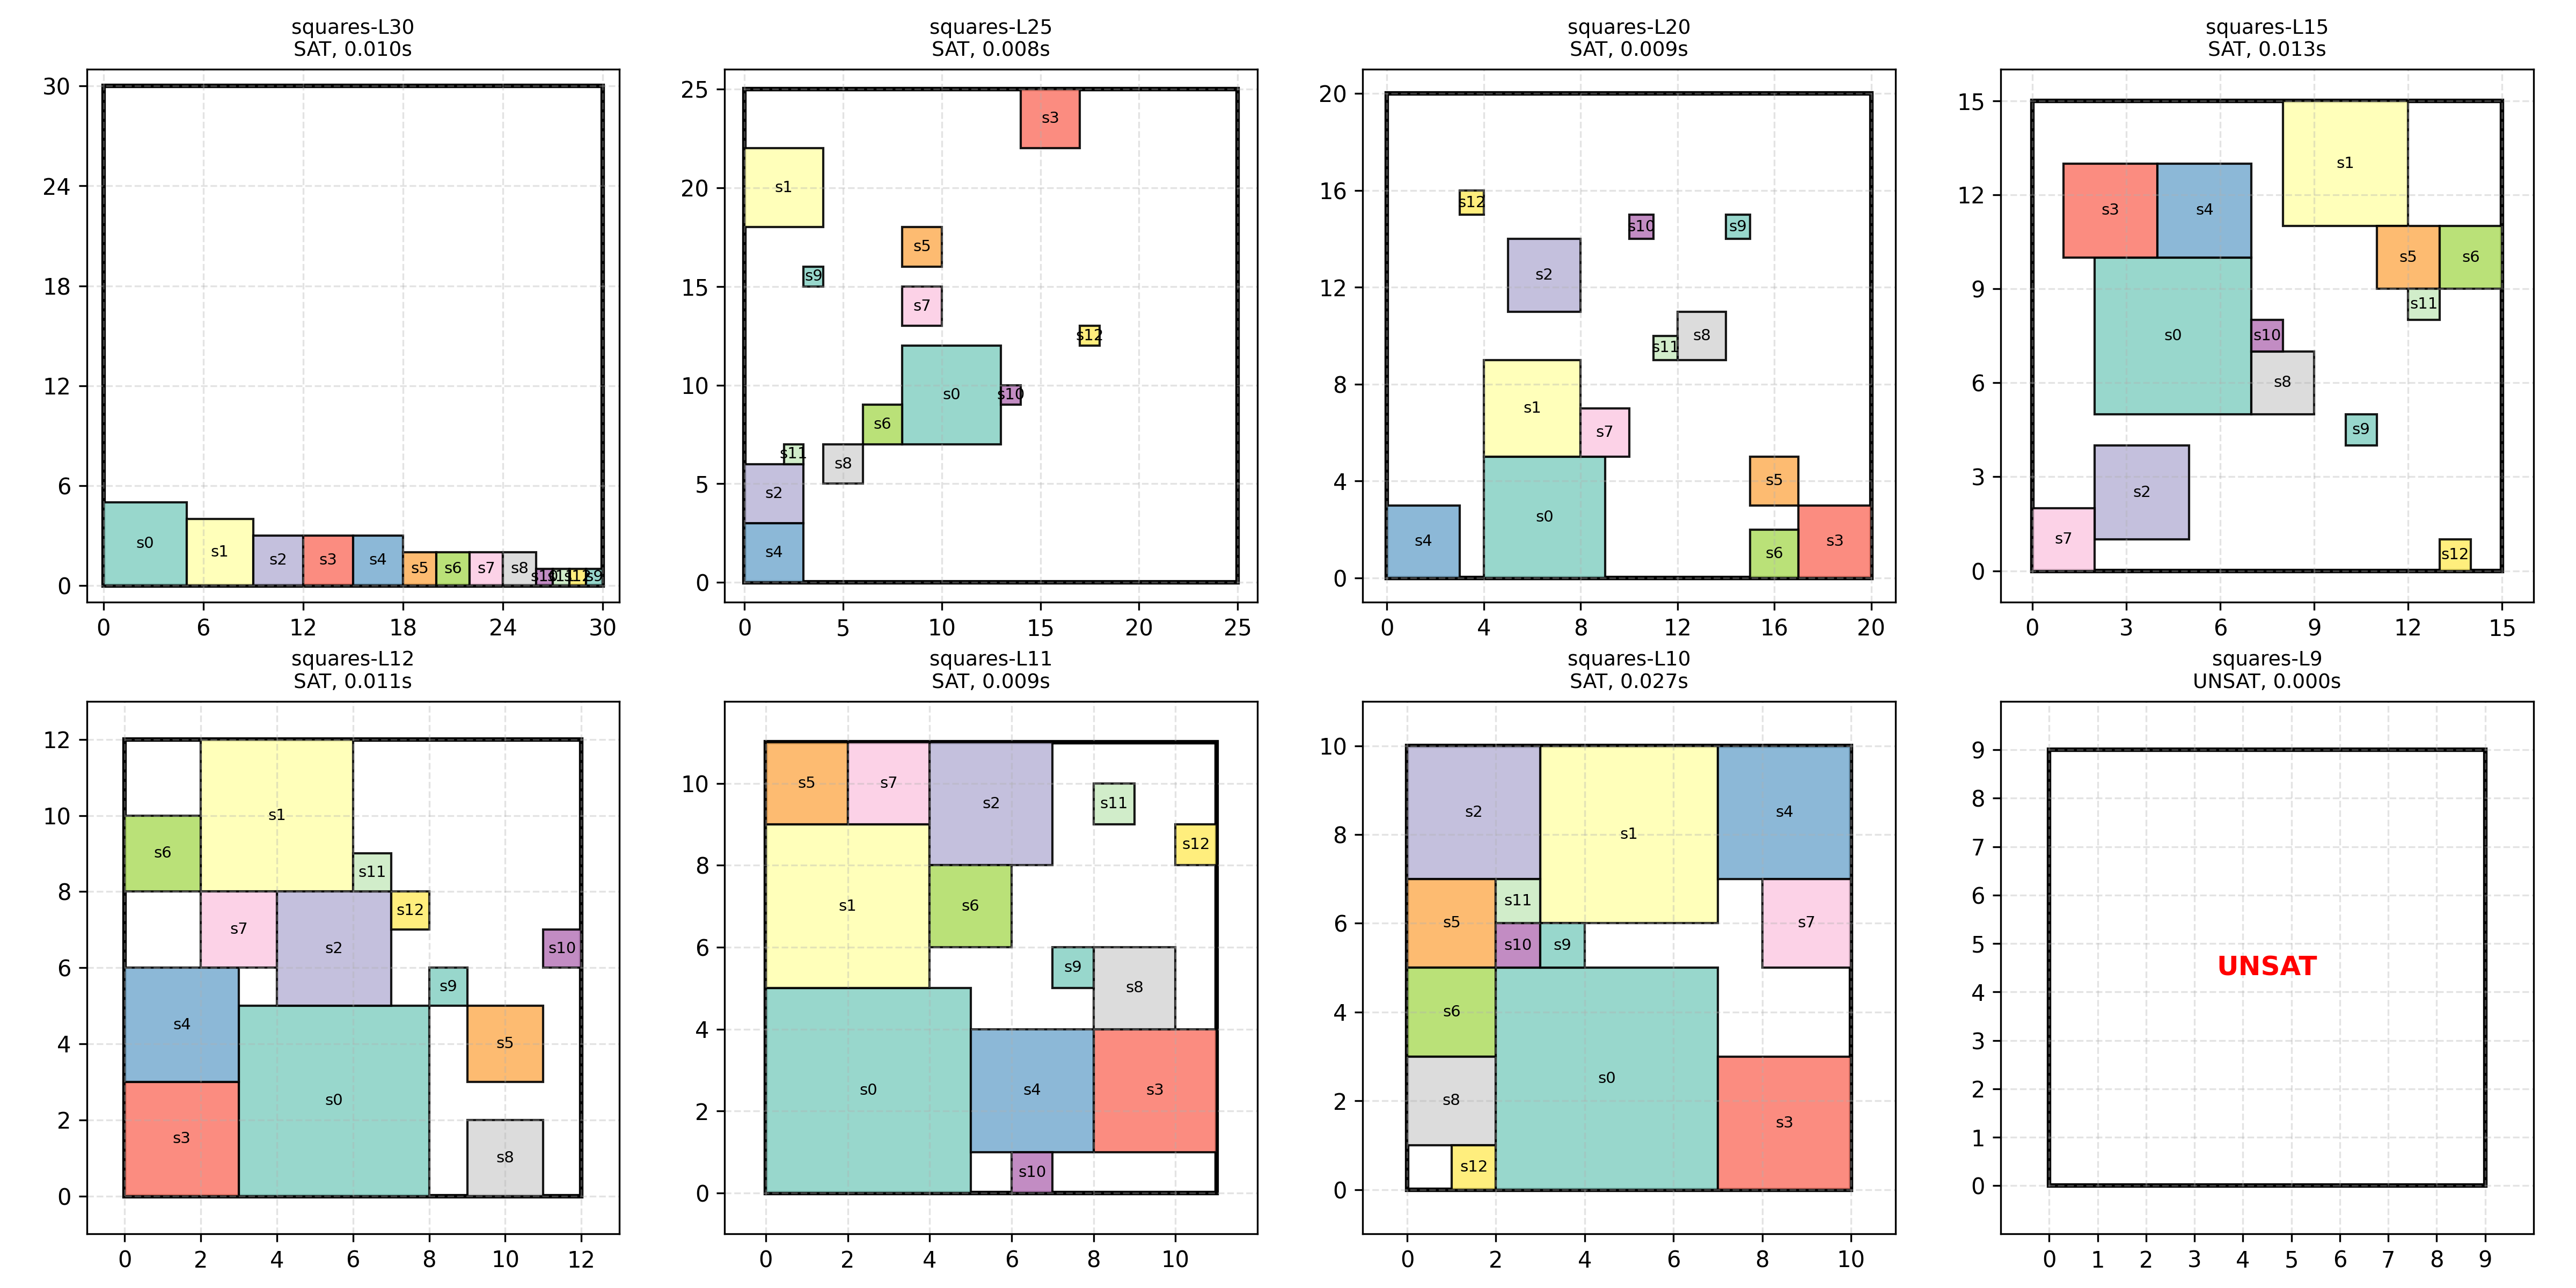
\includegraphics[width=0.95\textwidth]{../results/square_baseline_grid.png}
\caption{Z3-generated square baseline packings for several container sizes.}
\end{figure}

\subsection{Rectangle and Rotation Experiments}

The rectangle experiments use the same container and piece set under two modes:
\texttt{rectangles\_no\_rotation} and \texttt{rectangles\_rotation}. This
comparison isolates the effect of adding Boolean rotation variables. Rotation
can make otherwise impossible instances feasible, but it also increases the
solver's search space. The included rotation witness has two \(3\times2\)
rectangles in a \(5\times3\) container: without rotation the instance is UNSAT,
while with rotation one rectangle can rotate and the instance becomes SAT.

\begin{table}[h]
\centering
\begin{tabular}{rrllrr}
\toprule
Pieces & Density & No rotation & Rotation & No-rot time & Rot time \\
\midrule
4 & 0.6333 & SAT & SAT & 0.0026 & 0.0028 \\
5 & 0.7667 & SAT & SAT & 0.0034 & 0.0048 \\
6 & 0.8500 & SAT & SAT & 0.0050 & 0.0074 \\
7 & 0.9250 & SAT & SAT & 0.0067 & 0.0079 \\
8 & 0.9917 & UNSAT & SAT & 0.0068 & 0.2816 \\
\bottomrule
\end{tabular}
\caption{Rectangle experiments in a \(12\times10\) container. The \(n=8\)
case demonstrates that allowing rotation can change the answer from UNSAT to
SAT, at the cost of a larger search space.}
\end{table}

\begin{figure}[H]
\centering
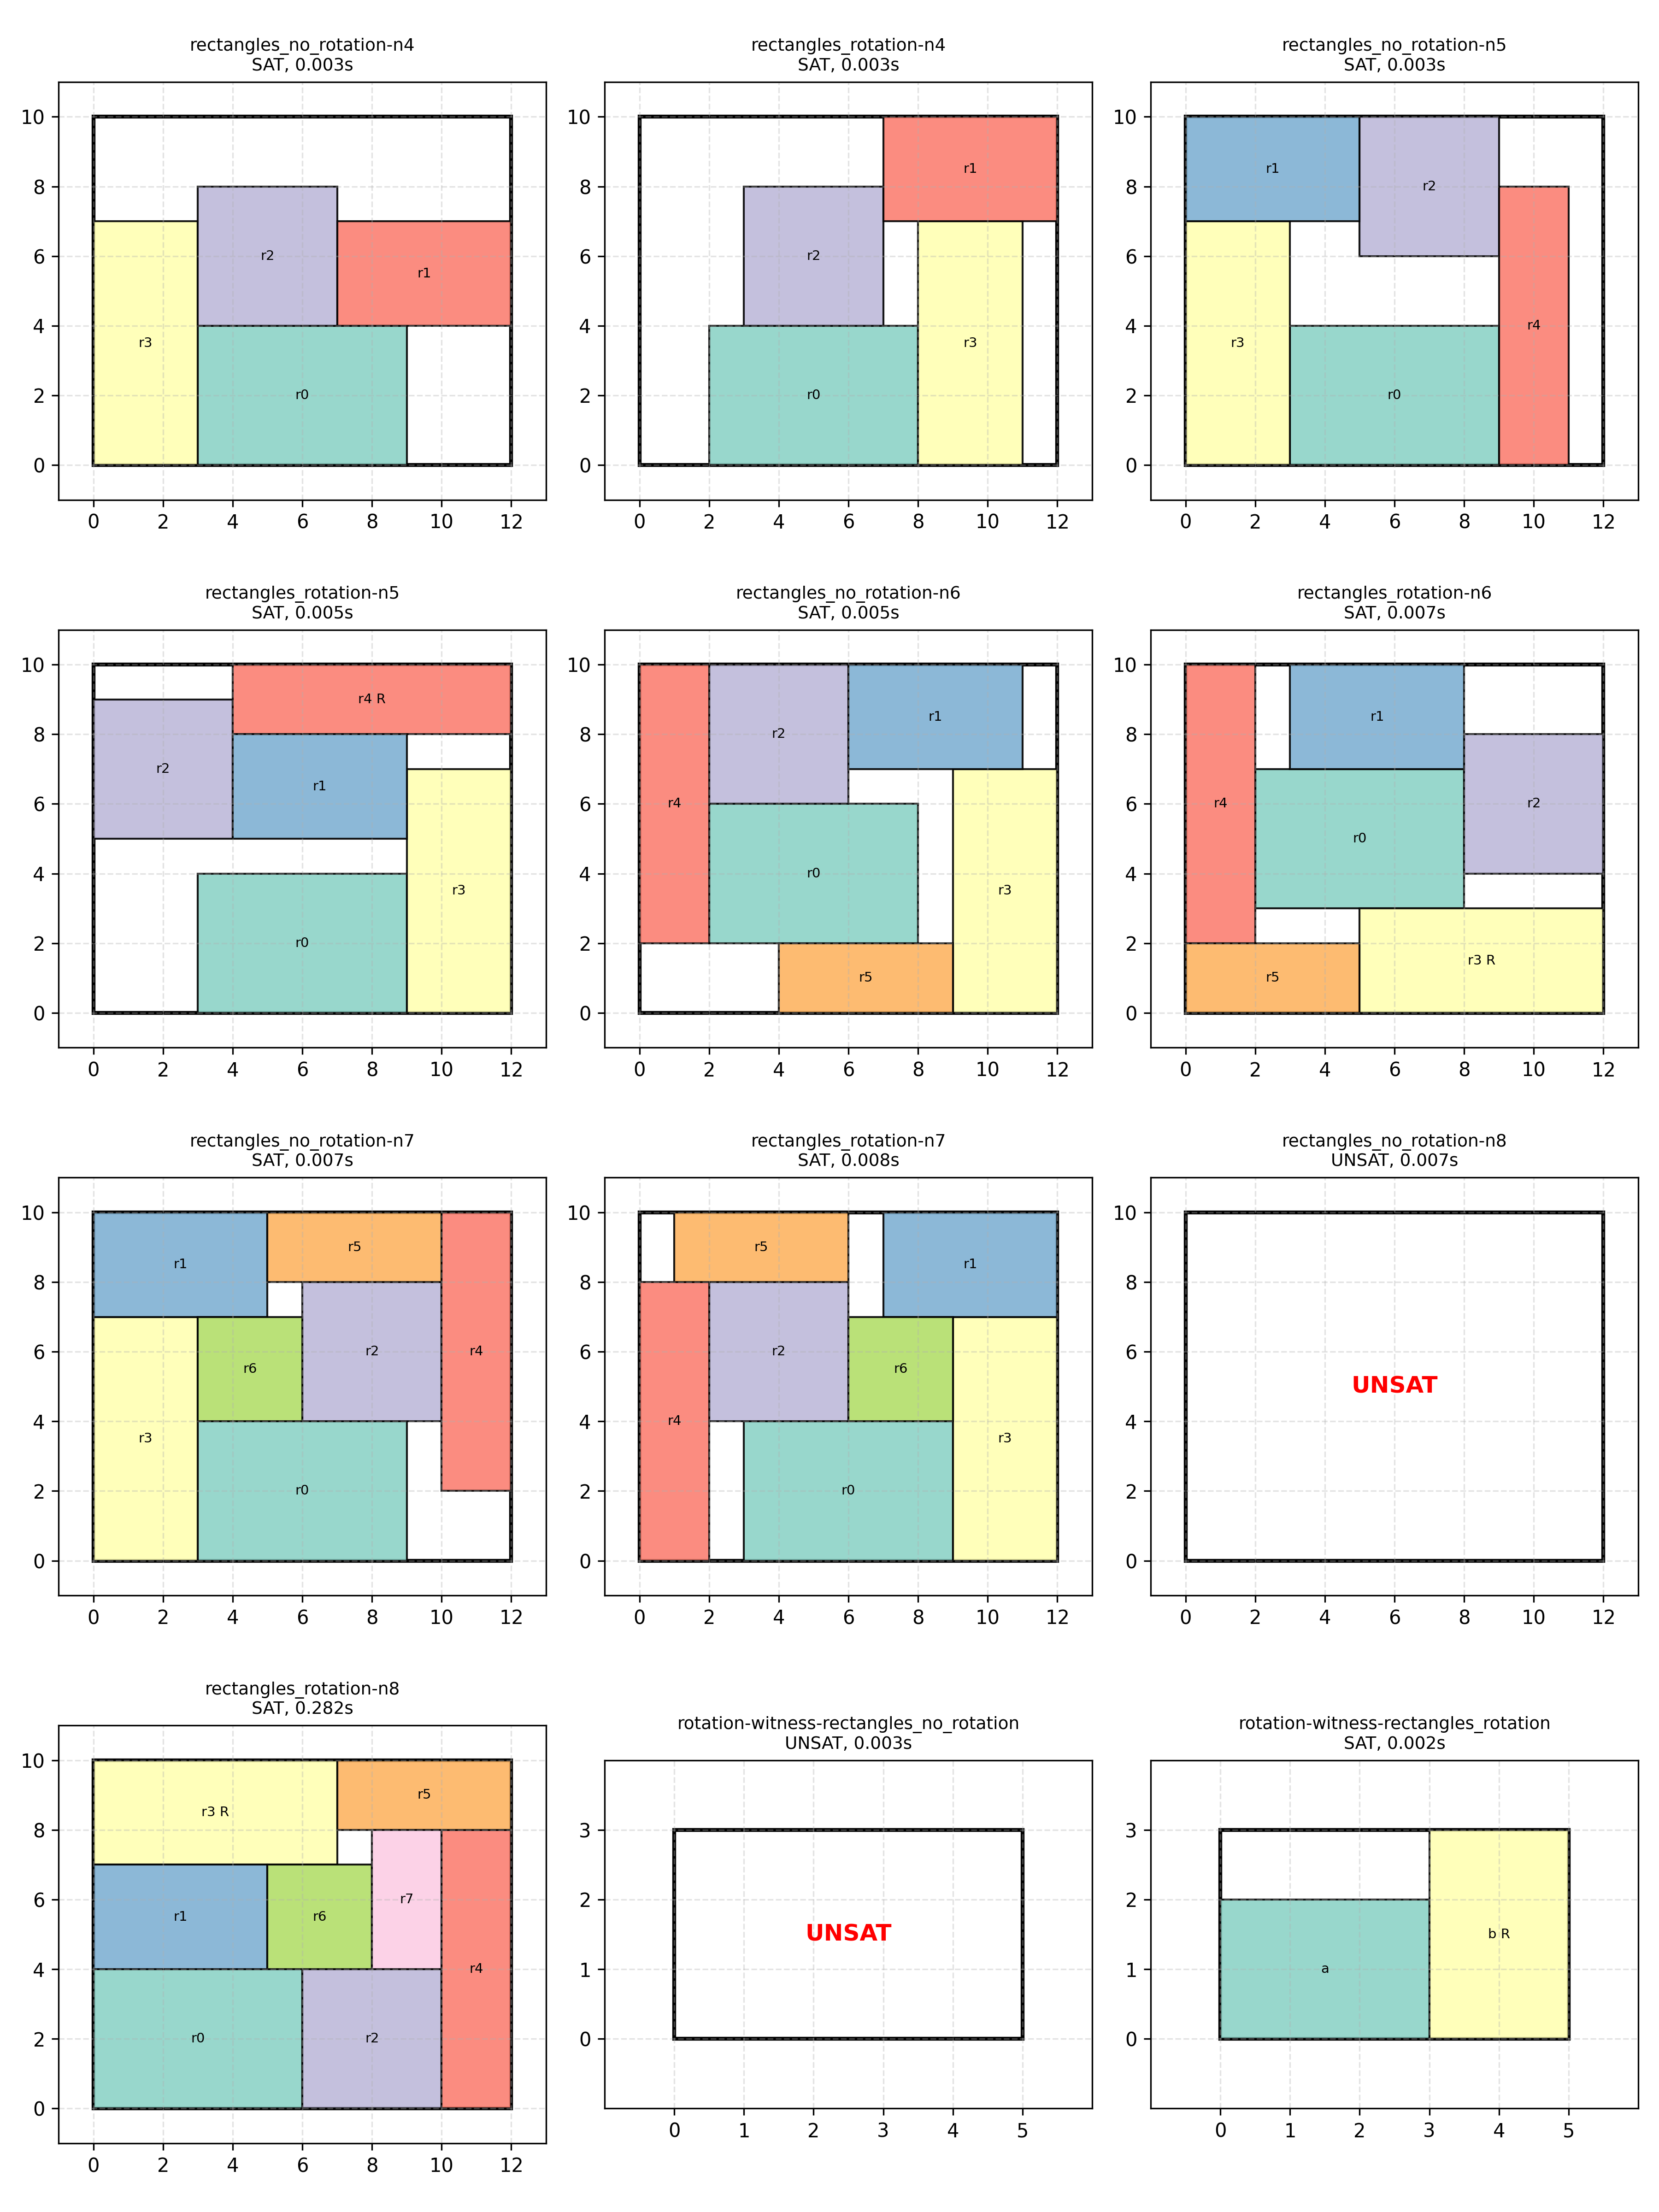
\includegraphics[width=0.95\textwidth]{../results/rectangle_experiments_grid.png}
\caption{Rectangle experiments comparing fixed orientation and optional
rotation.}
\end{figure}

\subsection{Density Scaling}

The random experiments use deterministic seeds and gradually increase the
number of rectangles inside a fixed container. The key input dimensions are the
number of pieces, the container size, the distribution of piece dimensions, the
density ratio, and whether rotation is enabled. We expect instances near the
feasibility boundary to be harder than very sparse or trivially impossible
instances.

\section{Input Instances and Dimensions}

The tool supports both Python-generated benchmark instances and a JSON input
format containing the board size, piece dimensions, and optional solver
settings. A JSON instance contains a container width and height, a list of
pieces with integer dimensions, and settings such as timeout and symmetry
breaking.

The main input dimensions are:
\begin{itemize}
    \item \(n\), the number of pieces;
    \item \(C_W,C_H\), the container dimensions;
    \item the distribution of square or rectangle dimensions;
    \item the density ratio \(\sum_i w_i h_i / (C_W C_H)\);
    \item whether rotation is enabled.
\end{itemize}

We expect the solver to become slower as \(n\) increases because the number of
pairwise non-overlap constraints grows as \(\binom{n}{2}\). We also expect
instances near the feasibility boundary to be harder, because the solver has
less free space and must reason about many more conflicting placements.

\section{Team Contributions}

Changqing Li focused on the SMT reduction, including the coordinate encoding,
rotation variables, and correctness argument. Fei Keng focused on the Python
implementation, deterministic test-case generation, and visualization outputs.
Grant O'Connor focused on the background research and experimental writeup,
including the explanation of why packing is relevant to areas such as VLSI
layout, manufacturing, and logistics.

\section{Conclusion}

This project demonstrates how NP-hard packing problems can be solved through a
SAT/SMT reduction. For integer square packing, the SAT encoding uses Boolean
variables for legal placements, while our implementation uses a more compact
SMT encoding with integer coordinate variables. We then extend the same
encoding to rectangle packing with optional rotation by adding effective width
and height expressions controlled by Boolean rotation variables. In all modes,
satisfiability corresponds exactly to the existence of a valid packing. The
tool supports JSON inputs, reproducible experiments, CSV summaries, and
visualizations suitable for analyzing solver behavior.

\bibliographystyle{plain}
\bibliography{references}

\end{document}
